\subsection{Skeleton Creation}
\label{sec:skeleton}

%\todo{why need a skeleton. We divide the whole inference
%into three tasks}


A query skeleton is an incomplete SQL query
that captures the basic structure of the result query.
It consists of three parts: query tables,
join conditions, and projection columns.
To create it, \ourtool performs a simple scan over
the examples, and uses several heuristics to determine
each part.
%Other elements in the query, such as query conditions
%and aggregate functions, will be determined in
%the next step.

%A query skeleton captures the most basic structure of
%a SQL query; creating it is the first step of synthesizing
%a complete query. \ourtool performs a simple scan over
%the examples, and employs several heuristics to determine
%the table set, joining columns, and project columns.

%\todo{why heuristics. the source of PSPACE}

%\item
\vspace{1mm}
{\textbf{Determining query tables.}} 
A typical end-user is often unwilling to provide more than enough
example input. Thus, we assume every example input table
is used (at least once) in the result query.
By default, the query tables are all example input tables.
Yet it is possible that one input table will be
used multiple times in a query. \ourtool does not forbid this case;
it uses a heuristic to estimate the query tables.
If the same column from an input table appears $N$ ($N >$ 1) times in the
output table, it is highly likely that the input table
will be used multiple times in the query, such
as being joined with different tables.
%be joined with other tables multiple times and forms 
%different values on the same projection column.
Thus, \ourtool replicates the input table $N$ times in
the query table set.
%the same number of times.\todo{xx}

%The rationale behind this heuristic is that if a table column
%appears multiple times in the output, it may indicate that the
%table would be joined multiple times.



%\item
\vspace{1mm}
%\noindent
{\textbf{Determining join conditions. }} There
are many ways to join all query tables; enumerating
all possibilities may yield a large number of
join conditions and is feasible in practice. 
To determine the most likely join conditions among them,
\ourtool uses two rules to repeatedly join
two different tables in the query tables,
until all tables get joined.
First, \ourtool seeks to join
tables on columns with the
same name and the same data type. For example,
in Figure~\ref{fig:motivating}, the \CodeIn{student} table
is joined with the \CodeIn{enrolled} table on the
\CodeIn{student\_id} column, which exists in both
tables and has the same data type.
If such columns do not exist,
\ourtool uses the second rule to
join tables on columns with the same data type
(even with different names).
For example, suppose the column name \CodeIn{student\_id}
in the \CodeIn{student} table of Figure~\ref{fig:motivating}(a)
is changed to \CodeIn{student\_key}, \ourtool will no longer
find a column with the same name and data type in
table \CodeIn{student} and table \CodeIn{enrolled}. In this case,
\ourtool will identify three possible join conditions
by only considering columns with the same data type:
\CodeIn{student\_key = student\_id}, \CodeIn{student\_key = course\_id},
and \CodeIn{student\_key = score}; and then creates 
three skeletons, each of which uses one join condition. 

%\item
%\vspace{1mm}
%\noindent 
{\textbf{Determining projection columns.}} \ourtool
scans each column in the output table, and checks whether
the column name appears in an input table.
If so, \ourtool uses the matched column from the input
table as the projection column in the skeleton.
Otherwise, the output column must be created by using an aggregate.
Take the output table in Figure~\ref{fig:motivating} as an
example, \ourtool determines that the \CodeIn{name} column
is from the \CodeIn{student} table and
the \CodeIn{max\_score} column is created by using
an aggregate over some column.


%Note that, if multiple columns (with the same name and data type)
%in different input tables has the same name as a column in the output table, \ourtool
%can safely uses an abitrary one; since columns with the
%same name and data type will be used in join conditions and
%are guaranteed to have the same value in the jo
%\todo{xx}



%which the querying result would be projected, our technique checks whether each output
%table column name appears in any input tables. If so, we used the matched column
%from the input table as the output column.  Our technique keeps track of those aggregation columns
%and search for proper aggregates in the next phase (Section~\ref{sec:agg_search}). 
%\todo{check the values in the output column}

\vspace{1mm}



%\begin{figure*}[t]
    \centering
    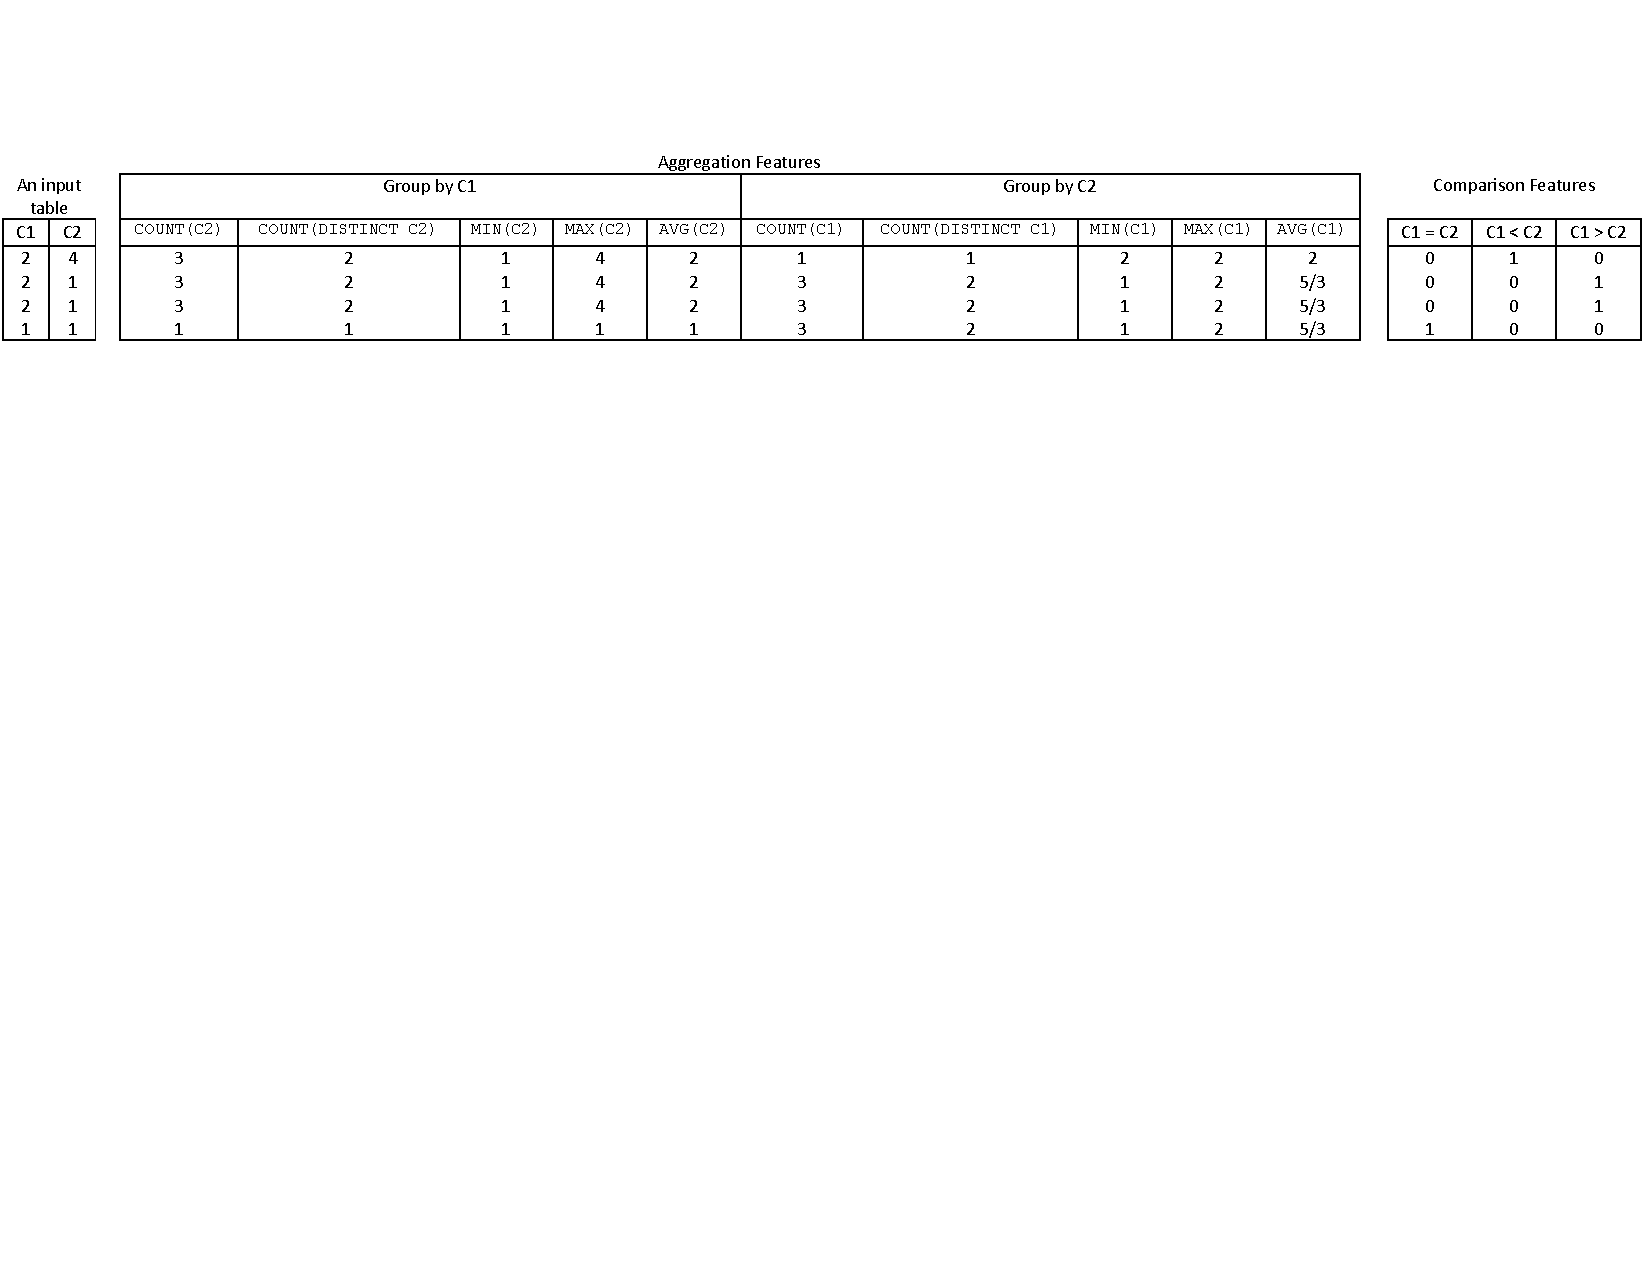
\includegraphics[scale=0.68]{featurex}
    \vspace{-7mm}
	\caption{Illustration of two additional features
    added by \ourtool. (Left) An example input table with
    two columns: C1 and C2. (Center) The aggregation features added by
    \ourtool for the input table. (Right) The comparison features
    added by \ourtool for the input table.
    Take the first row in the input table as an example,
    when grouping the table by column C1 (with value 2), the number
    of values in the C2 column is 3; the  number of
    distinct values in the C2 column is 2; the minimal value
    in the C2 column is 1, the maximal value in the C2 column
    is 4, and the average value in the C2 column is 2. Similar
    results can be computed if the table is grouped by the C2
    column.
}
	\label{fig:features}
\end{figure*}


\begin{figure}[t]
	\centering
		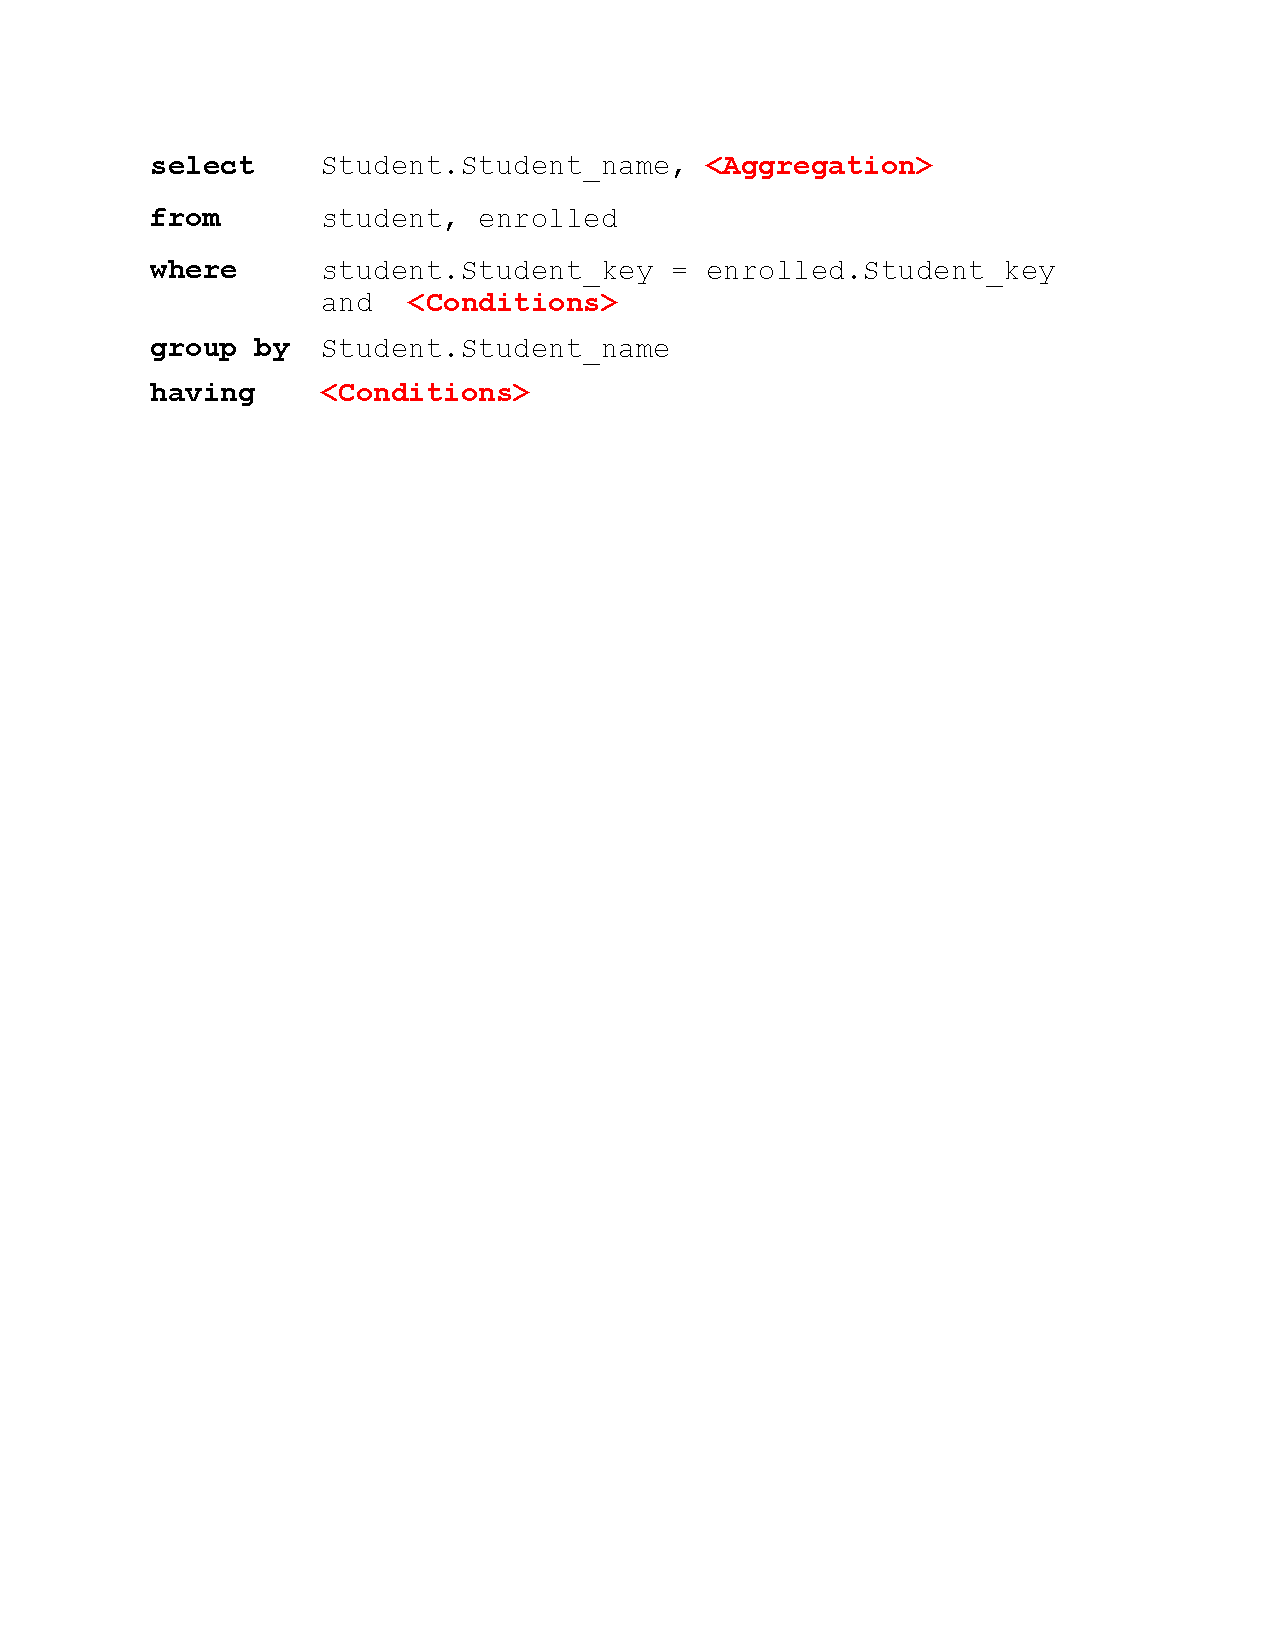
\includegraphics[width=0.45\textwidth]{sql_skeleton.pdf}
        \vspace{-3mm}
	\caption{A query skeleton created for the motivating example
in Figure~\ref{fig:motivating}. The missing parts (in red) will
be completed in Section~\ref{sec:completion}.}
	\label{fig:skeleton}
\end{figure}


For an example input and output pair,
depending on the number of join conditions,
\ourtool may create multiple skeletons,
which share the same query tables and
projection columns, but differ in the join condition.
For the example in Figure~\ref{fig:motivating},
\ourtool creates one query skeleton shown in Figure~\ref{fig:skeleton}.

%The number of created skeletons equals to the number of
%possible join conditions, and each skeleton only differs
%n its join conditions.  
%In this skeleton,  three unknown structures represented by
%$<$Aggregation$>$ or $<$Conditions$>$ are in red, and
%will be filled in the next phase. \todo{revise text}



% which indicates aggregation and group by.

%After determining the table set and joining columns,
%the next step is to identify potential column names on which the result would be projected. If a
%column in the output table  does not appear in any input table's column list, this output column must
%be produced by aggregation. Our algorithm keeps track of these columns and appends a \CodeIn{group by} ... \CodeIn{having} ...
%clause to the query skeleton.

%\end{itemize}

%In summary, this step infers three parts as a query skeleton: tables used in constructing a SQL query, joining conditions
%to connect the input tables, and a list of columns to project the output results.

%It is worth noting that the results obtained from the above steps are not \textit{safe} in
%terms that they may miss some valid SQL queries. 

%We made the above assumption for the sake of tractability,
%since in theory, the bound of table number in a SQL query is $O(n_t!)$, where $n_t$ is the number of given tables;
%while the bound of possible number of join is $O(c_t^2)$ and the bound of the number of conditions is $O(n_t!n_tc_t^2)<O(n_t^3c_t^2)$.

%\subsubsection{Inferring Output Table Schema}

%Lacks schema


%while the bound of possible number of join is $O(c_t^2)$ and the bound of the number of conditions is $O(n_t!n_tc_t^2)<O(n_t^3c_t^2)$.


